%%%%%%%%%%%%%%%%%%%%%%%%%%%%%%%%%%%%%%%%%%%%%%%%%%%%%%%%%%%%%%%%%%%%%%%%%%%%%%%%%%%%%
%																					%
%	TRABAJO: Paper Redes de Petri con Tiempo										%
%																					%
%		Titulo: 	Ejecucion de Redes de Petri con Tiempo							%
%																					%
%		Autores:	Julian Nonino													%
%					Carlos Renzo Pisetta											%
%					Orlando Micolini												%
%																					%
%	Seccion: IP core																%	
%	Archivo: ip_core.tex															%
%																					%
%%%%%%%%%%%%%%%%%%%%%%%%%%%%%%%%%%%%%%%%%%%%%%%%%%%%%%%%%%%%%%%%%%%%%%%%%%%%%%%%%%%%%
%	REVISIONES																		%
%																					%
%		19/10/2012																	%
%			Julian Nonino															%
%				Creacion de este archivo											%
%		04/04/2013																	%
%			Renzo Pisetta															%
%				Modifica															%
%																					%
%%%%%%%%%%%%%%%%%%%%%%%%%%%%%%%%%%%%%%%%%%%%%%%%%%%%%%%%%%%%%%%%%%%%%%%%%%%%%%%%%%%%%

\section{IP cores}

			La arquitectura del procesador de Redes de Petri ya existente se expande para soportar las nuevas sintaxis,se 
		agregan estructuras de datos necesarias.
		
\begin{figure}[h]
			\centering
			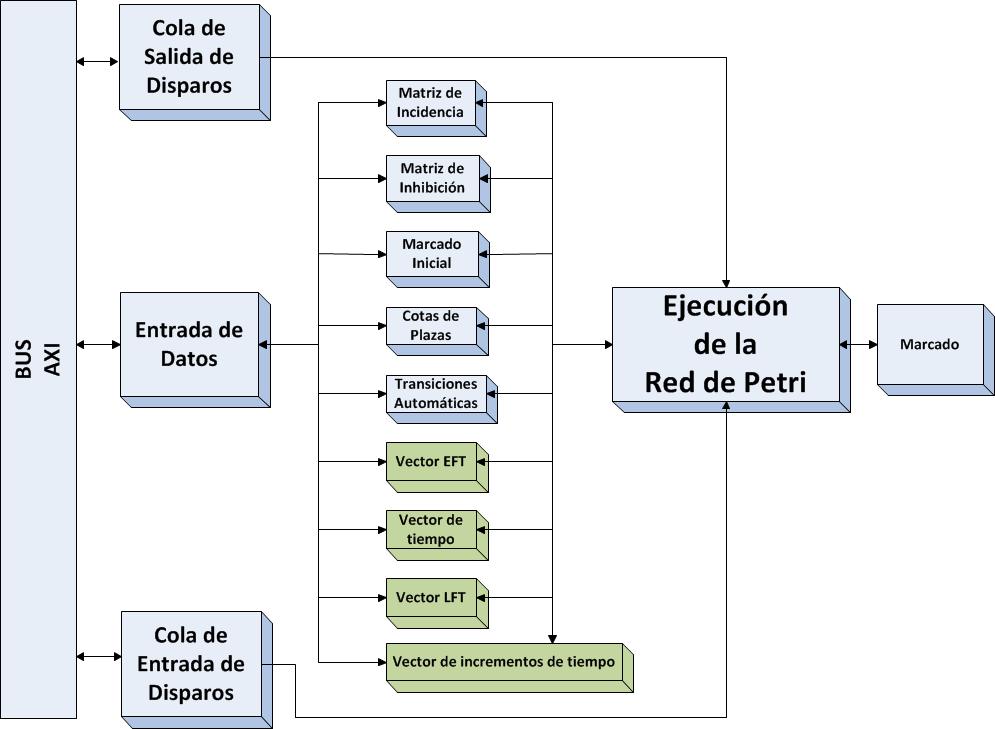
\includegraphics[width=3in]{./img/diseno33}
			\caption{Arquitectura del Procesador de Redes de Petri con Tiempo}
			\label{fig:diseno33}
\end{figure}
	\begin{itemize}
		  	\item Vector \textbf{\emph{Earlier Firing Time (EFT)}}.
		  	\item Vector de \textbf{\emph{marcas temporales}}.
		  	\item Vector \textbf{\emph{Latest Firing Time (LFT)}}.
		  	\item Vector de \textbf{\emph{escala de incrementos de tiempo}}.
		\end{itemize}
		Los cuatro vectores tienen como cantidad de elementos el n�mero de transiciones. Los 
		tres primeros tienen un tama�o de elementos parametrizable pero por defecto tienen 
		48 bits. El vector de escala de incrementos de tiempo, por defecto toma el un tama�o 
		de elementos de 5 bits.

\subsection{Algoritmo de Ejecuci�n con Redes de Petri con Tiempo}
	Basados en la teoria descripta se creo un algoritmo de ejecuci�n de disparos en una red de petri que se describe a continuaci�n es sintetizable en hardware y requiere 
	�nicamente 2 ciclos de reloj para ejecutar todos los pasos y a la vez permita un dise�o parametrizable en cuanto al tama�o y cantidad de elementos que soporte.
	
	\begin{enumerate}
	\item Espera de disparo en Cola de entrada de disparos.
	\item Llegado el disparo se calcula un vector binario de longitud cantidad de transiciones con un �nico 1 en el lugar correspondiente al n�mero de disparo, en funci�n del n�mero de transici�n que contenga. Este vector se utiliza para incrementar los contadores de disparos.
		Son considerados disparos en espera.
	\item Se calcula todos los posibles resultados para todos los disparos, hayan sido pedidos o no para confeccionar una matriz resultado donde cada columna Ci representa el nuevo marcado si la transici�n Ti  se disparara.
	\item Se crea una matriz de signos auxiliar con los signos correspondientes a cada elemento de la matriz resultado. 
	\item Se crea una matriz de inhibici�n auxiliar en funci�n del marcado actual y la Matriz de Inhibici�n determinando las plazas con arcos inhibidores que tienen tokens.
	\item Se crea una matriz de cotas en funci�n de la matriz resultados y las cotas de las plazas determinando cual fue superada para cada plaza por cada posible resultado
	\item Se crea un vector en el cual cada elemento corresponde a una columna de la matriz de signos y determina si esa transici�n es o no posible en funci�n si alg�n elemento de su resultado es negativo.
	\item Se crea un vector en el cual cada elemento corresponde a una columna de la matriz de inhibici�n y determina las transiciones que no pueden ser disparada debido a arcos inhibidores.
	\item Se crea un vector en el cual cada elemento corresponde a una columna de la matriz de cotas el cual determina que transiciones no pueden ser disparadas debido a que provocar�an superar las cotas de las plazas.
	\item En funci�n de los vectores creados en los puntos 7, 8 y 9 se crea un vector que determina las transiciones sensibilizadas. 
	\item Se genera un vector en el cual cada elemento corresponde a la transici�n de igual �ndice y se verifica que vector de tiempo correspondiente se encuentre entre el EFT y LFT para determinar si la transici�n se puede ejecutar en funci�n del tiempo
	\item Se genera un vector en funci�n de lo obtenido en los puntos 10 y 11 determinando que disparos son posibles.
	\item Para determinar las transiciones a disparar se unen los disparos pendientes y las transiciones autom�ticas. Luego en funci�n de los disparos posibles y que la cola de disparos de salida no est� llena se actualiza el marcado actual a partir del resultado obtenido en el punto 3 considerando la mayor prioridad al �ndice de mayor valor. 
	\item Se incrementa contador de cola de salida correspondiente a transici�n ejecutada.
	\item En cada clock de reloj se actualiza el vector de tiempo (contador saturado) de cada transici�n sensibilizada increment�ndolo seg�n el vector de incremento de tiempo correspondiente a partir de que la transici�n es sensibilizada.

\end{enumerate}	